%\glsresetall
\glsreset{cstp}
\glsreset{clumrct}
%%========-----------------------1.	Giải thuật tiến hóa đa nhân tố---------------------------============
Chương 2 trình bày bài toán \gls{clumrct}, bài toán \gls{cstp}, các ứng dụng và các nghiên cứu liên quan.

\section{Bài toán cây khung phân cụm} \label{chap_coso:sec:gioiThieuCayKhungPhanCum}
%\subsection{Bài toán tiến hóa đa nhân tố} \label{chap_coso:sec_mfea:subsec:baitoandanhanto}
Bài toán cây khung có chi phí nhỏ nhất (Mininum Cost Spanning Tree - MCST) trên đồ thị có trọng số là một trong các bài toán nổi tiếng trong lĩnh vực toán ứng dụng cũng như trong khoa học máy tính. Bài toán MCST được ứng dụng trong nhiều lĩnh vực thực tiễn như tối ưu hệ thống truyền thông, tối ưu hệ thống giao vận. Trong nghiên cứu lý thuyết, đã có rất nhiều biến thể của bài toán MCST (khi thay đổi hàm mục tiêu hoặc thêm các rằng buộc) được nghiên cứu như bài toán cây khung nhỏ nhất (Minimum spanning tree)~\cite{raidl_edge_2003, khuller1995balancing}, cây Steiner nhỏ nhất (Steiner minimum tree)~\cite{winter1997euclidean}, cây đường đi ngắn nhất (Shortest-path tree)~\cite{dial1979computational, khuller1995balancing} và cây khung với chi phí định tuyến (Minimum routing cost spanning tree)~\cite{julstrom2005blob}.

Tuy nhiên, trong nhiều ứng dụng mạng, các điểm đầu cuối có thể được chia vào các nhóm sao cho việc kết nối giữa các điểm đầu cuối trong cùng một nhóm có tính “cục bộ” nhằm đảm bảo tính hiệu quả và an toàn. Khi đó, cần phải tìm cây khung của đồ thị con của các đỉnh thuộc cùng một nhóm không chứa các đỉnh thuộc các nhóm khác. Cụ thể hơn, trong lĩnh vực nông nghiệp, con người từ rất sớm đã có nhu cầu tối ưu hệ thống dẫn nước tưới tiêu từ một giếng nước tới các ốc đảo trong sa mạc, trong mỗi ốc đảo lại cần tối ưu hệ thống dẫn nước tới các vị trí trồng cây. Trong lĩnh vực bưu chính và giao vận, các công ty thường có nhu cầu tối ưu vận chuyển thư từ hay hàng hóa từ trung tâm tới các tỉnh, rồi từ các tỉnh lại vận chuyển tới các huyện, xã.

Từ yêu cầu thực tiễn đó, một lớp các bài toán cây khung phân cụm đã được quan tâm nghiên cứu. Trong đó, bài toán \gls{clumrct} và bài toán \gls{cstp} là hai trong số nhiều các bài toán có vai trò quan trọng trong các ứng dụng thực tiễn và nhận được nhiều sự quan tâm của các nhà nghiên cứu. Bài toán CluMRCT giúp tìm ra một thiết kế hiệu quả để giảm thiểu chi phí vận chuyển và chi phí xử lý trung gian trong quá trình phân phối, đồng thời vẫn đảm bảo duy trì được những lợi thế về tính an toàn và hiệu quả mà mạng phân cụm đem lại, do cây khung tìm được vẫn duy trì sự phân cụm ban đầu của đồ thị đầu vào. Bài toán CluSPT có thể được áp dụng để giải quyết những yêu cầu thực tế về tối ưu những mạng phân cụm có một nút nguồn quan trọng. Cụ thể, trong các hệ thống tưới tiêu, nguồn nước có thể được coi là nút nguồn và một tiêu chí quan trọng cần xét đến khi thiết kế hệ thống tưới tiêu chính là khoảng cách từ nguồn nước tới các địa điểm khác trong hệ thống, hay nói cách khác là chi phí từ nút nguồn đến các nút khác trong mạng. Trong phân phối hàng hóa, nút nguồn có thể là xưởng sản xuất hoặc đầu mối phân phối hàng. Nói cách khác, khi tồn tại một nút trong mạng mà có giao tiếp nhiều với tất cả các nút còn lại thì một yêu cầu đặt ra chính là tối thiểu hóa tổng chi phí từ nút đó tới mỗi nút khác trong mạng. 

%%=================--------------------------------2.Các ký hiệu và định nghĩa---------------------------========================
\section{Các ký hiệu và định nghĩa} \label{chap_coso:sec:kyHieuVaDinhNghia}
	Cho đồ thị $G=(V, E, w)$ trong đó $V$ và $E$ lần lượt là tập đỉnh và tập cạnh của đồ thị; $w$ là ma trận trọng số cạnh của đồ thị. Ký hiệu:
\begin{itemize}
	\item Cạnh nối giữa đỉnh $u$ và đỉnh $v$ ký hiệu là $e=(u, v)$ và trọng số của cạnh ký hiệu là $w(u, v)$ hoặc $w(e)$.
	\item $V(G)$ và $E(G)$ là tập đỉnh và tập cạnh của đồ thị $G$.
	\item Cho trước tập các đỉnh $S \subseteq V$, $G[S]$  là đồ thị con của $G$ được cảm sinh bởi tập $S$. 
	\item Tập $R=\{R_1, R_2, \ldots,R_k\}$ được gọi là phân hoạch của $V$ nếu $R_1 \cup R_2 \cup \ldots \cup  R_k = V$ và $R_i \cap R_j = \emptyset, \forall i, j \in [1,k]$.
\end{itemize}

\begin{definition}[Chi phí định tuyến giữa hai đỉnh]
Cho G = (V, E, w) là một đồ thị vô hướng, liên thông, các cạnh có trọng số không âm. Chi phí định tuyến giữa hai đỉnh $u, v \in V$ trên cây khung T (ký hiệu $d_T$(u,v)) của đồ thị $G$ được tính bằng khoảng cách giữa hai đỉnh đó trên cây khung T.
\end{definition}

\begin{definition}[Chi phí định tuyến của cây khung]
Cho G = (V, E, w) là một đồ thị vô hướng, liên thông, các cạnh có trọng số không âm. Chi phí định tuyến c(T) của cây khung T được tính bằng công thức:
\[
	c(T)= \sum_{u,v \in V(T)} d_T(u,v)
\]
 trong đó $d_T(u,v)$ là chi phí định tuyến giữa hai đỉnh u và v trên cây khung T.
\end{definition}

\begin{definition}[Đồ thị phân cụm]
Cho $G = (V,~E,~w)$ là đồ thị vô hướng, liên thông, các cạnh có trọng số không âm. Nếu tồn tại tập phân hoạch $R=\{R_1, R_2,\ldots,R_k\}$ của $V$ thì $G$ được gọi là đồ thị phân cụm, tập $R_1, R_2, R_3,\ldots,R_k$ được gọi là các cụm (cluster) của đồ thị.
\end{definition}	
	
\begin{definition}[Cây khung phân cụm]
Cho đồ thị có trọng số cạnh $G = (V, E, w)$ trong đó các đỉnh được phân hoạch thành k cụm $R=\{R_1, R_2, \ldots,R_k\}$, một cây khung T của G là cây khung phân cụm nếu các cây con cảm sinh của T trên G cũng là cây khung.
\end{definition}

%\begin{definition}
%	Cho một đồ thị có trọng số cạnh G = (V, E, w) trong đó các đỉnh được phân hoạch thành k cụm R=\{$R_1, R_2, \ldots,R_k$\}, đỉnh $v \in R_i$ được gọi là đỉnh nguồn của một cụm $R_i$ nếu $v$ là đỉnh có cạnh nối với các đỉnh của các cụm khác.
%\end{definition}

\begin{definition}[H-Graph]
	Cho $G = (V,~E,~w)$ là đồ thị phân cụm. \text{H-Graph} là đồ thị được sinh ra từ đồ thị $G$ trong đó mỗi đỉnh của H-Graph tương ứng với một cụm trong đồ thị $G$, giữa 2 đỉnh của H-Graph có cạnh nối khi tồn tại ít nhất một cạnh nối giữa các đỉnh của các cụm tương ứng trong đồ thị $G$.
\end{definition}


%%===-------------------------2.Các ký hiệu và định nghĩa---------------------------========
\section{Phát biểu bài toán} \label{chap_coso:sec:phatbieubaitoan}
Có nhiều bài toán cây khung phân cụm được quan tâm nghiên cứu trong thời gian gần đây, tuy nhiên đồ án đi sâu nghiên cứu 2 bài toán \gls{clumrct} và \gls{cstp}.

\subsection{Bài toán Cây khung phân cụm có chi phí định tuyến nhỏ nhất} \label{chap_coso:sec_mfea:subsec:clumrct}
Cho $G = (V, E, w)$ là một đồ thị vô hướng, liên thông, các cạnh có trọng số không âm, tập phân hoạch của tập đỉnh $V$ là $R = \{R_1, R_2, R_3,\ldots,R_k\}$. Mục tiêu của bài toán \gls{clumrct} là tìm cây khung phân cụm $T$ cho đồ thị $G$ sao cho tổng chi phí định tuyến giữa tất cả các cặp đỉnh của $T$ là nhỏ nhất.

Mô hình toán học của bài toán \gls{clumrct} có thể được phát biểu như sau:

\noindent\textbf{Đầu vào:} Đồ thị phân cụm có trọng số cạnh $G = (V, E, w)$ và một phân hoạch $R = \{R_1, R_2, R_3,\ldots,R_k\}$ của $V$\\
\textbf{Đầu ra:} Một cây khung phân cụm $T$ của $G$ sao cho chi phí định tuyến $c(T)$ là nhỏ nhất. 


Đồ án này xem xét đồ thị đầu vào là đơn đồ thị liên thông vô hướng $G$ có tập đỉnh $V$, tập cạnh $E$, hàm trọng số cạnh $w$.

\renewcommand{\scalefigure}{0.6}
\begin{figure}[htbp]
	\centering		
	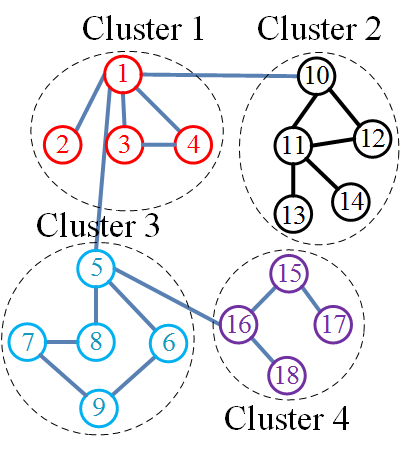
\includegraphics[scale=\scalefigure]{Pictures/CluMRCT/CluMRCT.png}
	\centering
	\caption{Cây khung phân cụm của bài toán CluMRCT cho đồ thị gồm 4 cụm và 18 đỉnh}
	\label{fig:vi_du_CluMRC}
\end{figure}

Hình \ref{fig:vi_du_CluMRC} minh họa cây khung phân cụm cho bài toán \gls{clumrct} của đồ thị đầu vào gồm 4 cụm, 18 đỉnh. Trong đó, các đỉnh thuộc một cụm nằm trong cùng một hình oval nét đứt.

\subsection{Bài toán Cây phân cụm đường đi ngắn nhất} \label{chap_coso:sec_mfea:subsec:cstp}
Bài toán \gls{cstp} được phát biểu như sau:

Cho một đơn đồ thị vô hướng $G = (V, E, w)$, một phân hoạch $R = \{R_1, R_2, R_3,\ldots,R_k\}$ của $V$ và đỉnh nguồn $s \in V$. Mục tiêu của bài toán \gls{cstp} là tìm một cây khung $T$ của đồ thị $G$ sao cho:
\begin{itemize}
	\item Với mỗi cụm $R_i (i=1,\ldots, k)$, đồ thị con $T[R_i]$ là một đồ thị liên thông.
	\item Tổng chi phí định tuyến giữa đỉnh nguồn và mỗi đỉnh $\sum_{v \in V(T)} d_T (s,v) \rightarrow$ min.
\end{itemize}

\renewcommand{\scalefigure}{0.6}
\begin{figure}[htbp]
	\centering		
	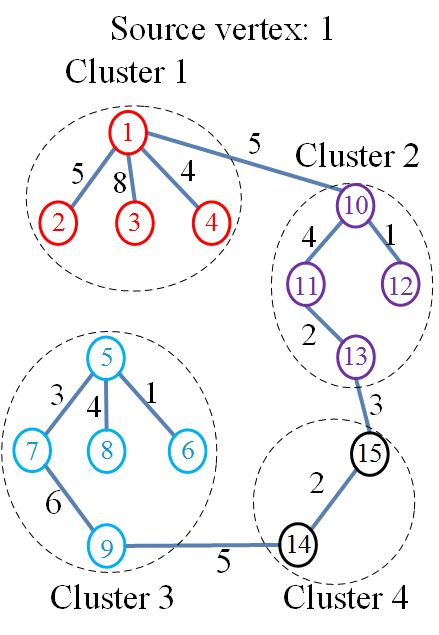
\includegraphics[scale=\scalefigure]{Pictures/CSTP/CSTP.png}
	\centering
	\caption{Cây khung phân cụm của bài toán \gls{cstp} cho đồ thị gồm 4 cụm và 15 đỉnh}
	\label{fig:vi_du_CSTP}
\end{figure}

Hình \ref{fig:vi_du_CSTP} minh họa một cây phân cụm của bài toán \gls{cstp} với đồ thị đầu vào gồm 15 đỉnh, 4 cụm và đỉnh 1 là đỉnh nguồn. Chi phí  của cây khung phân cụm là 186


%%=========--------------------------3. Các nghiên cứu liên quan---------------------------===============
\section{Các nghiên cứu liên quan} \label{chap_coso:sec:cacNghienCuuLienQuan}
\glsreset{clumrct}
\glsreset{cstp}
\glsreset{mfea}
Các bài toán liên quan đến các đỉnh được phân vào các cụm của đồ thị đã được biết đến từ những năm 70 của thế kỷ trước. Một trong các bài toán liên quan tới các đỉnh được phân cụm được nghiên cứu sớm nhất là bài toán \gls{clutsp}~\cite{bao_improved_2012, helsgaun_solving_2011, mestria_grasp_2013} - một biến thể của bài toán tối ưu tổ hợp nổi tiếng \gls{tsp} \cite{reinelt1994traveling}. Hiện nay, xuất phát từ yêu cầu cần tối ưu hệ thống mạng, bài toán cây phân cụm (clustered tree problems) nhận được nhiều sự quan tâm nghiên cứu.

Một trong các bài toán nhận được nhiều sự quan tâm nhất là bài toán \gls{clusteinertp}~\cite{wu_clustered_2015} - một biến thể của bài toán \gls{stp}~\cite{ihler_class_1999, winter1997euclidean}. Trong bài toán \gls{clusteinertp} các đỉnh cũng đươc chia vào các cụm, bài toán \gls{stp} là bài toán \gls{clusteinertp} nếu các cụm không có phần tử chung~\cite{wu2014clustered}. Trong \cite{wu_clustered_2015}, dựa trên kết quả thực nghiệm, các tác giả B. Y. Wu và C. W. Lin đã chỉ ra rằng tỉ lệ Steiner nằm trong khoảng (3,4) đem đến những kết quả có lợi nhất và từ đó đề xuất một giải thuật gần đúng cho bài toán \gls{clusteinertp} . Giải thuật này chuyển bài toán ban đầu về một bài toán cây Steiner sao cho cây Steiner tìm được không có đỉnh Steiner nào thuộc vào cây cục bộ của các cụm. Giải thuật được đề xuất giải có độ phức tạp đa thức.

Một biến thể khác của bài toán cây phân cụm, bài toán \gls{clumrct}~\cite{lin_minimum_2016}, trong nghiên cứu của mình các tác giả đã chỉ ra rằng bài toán \gls{clumrct} là NP-Khó nếu \gls{clumrct} có ít nhất 2 cụm. Nghiên cứu cũng đã đề xuất một giải thuật xấp xỉ cận tỉ lệ là 2 (2-approximation) để giải bài toán \gls{clumrct} bằng cách tạo đồ thị gồm 2 mức dựa trên cây khung R-star (R-star spanning tree) và dựa trên hai đặc trưng của cây khung \text{R-star}: một cây khung R-star với chi phí định tuyến nhỏ nhất có thể được tạo trong $O(n^2)$ với n là số đỉnh của bài toán và tồn tại một cây khung R-star với chi phí lớn nhất gấp 2 lần chi phí của lời giải tối ưu của bài toán \gls{clumrct}.


Gần đây, tác giả D'Emidio và các cộng sự \cite{demidio_clustered_2016} đã nghiên cứu một dạng khác của bài toán cây khung phân cụm, bài toán \gls{cstp}. Bài toán \gls{cstp} xuất hiện nhiều trong các ứng dụng cần tối ưu về thiết kế mạng, kết nối hệ thống cáp TV và hệ thống cáp quang. Trong nghiên cứu của mình nhóm tác giả đã đề xuất một giải thuật gần đúng (approximation algorithm - AAL) để giải bài toán \gls{cstp}. Ý tưởng chính của giải thuật AAL lần lượt tìm cây khung nhỏ nhất cho đồ thị con được cảm sinh từ tập đỉnh của mỗi cụm và đồ thị được nhận được bằng cách coi mỗi cụm là một đỉnh.

Như đã đề cập tới ở trong chương \ref{Chap_CoSoLyThuyet}, hướng tiếp cận sử dụng giải thuật gần đúng sẽ phù hợp hơn khi sử dụng giải các bài toán NP-Khó với dữ liệu đầu vào có kích thước lớn. Đối với các giải thuật gần đúng, giải thuật \gls{mfea} nổi lên như một giải thuật hiệu quả trong việc ứng dụng giải nhiều lớp bài toán khác nhau, đặc biệt các ứng dụng có hạn chế về tài nguyên sử dụng. Một trong các thế mạnh của giải thuật \gls{mfea} so với giải thuật GA là \gls{mfea} có thể tìm lời giải đồng thời của nhiều bài toán khác nhau nhưng chỉ sử dụng một mã hóa cá thể duy nhất cho tất cả các bài toán. Chính vì thế cho nên khi sử dụng giải thuật \gls{mfea}, lời giải của từng bài toán nhận được trên cơ sở thông tin của cá thể trong không gian \gls{uss}. Do đó, để sử dụng giải thuật \gls{mfea}, một trong các bước quan trọng cần phải giải quyết là tìm ra quy tắc biến đổi từ cá thể trong không gian \gls{uss} thành lời giải của từng bài toán. 

Hiện nay, giải thuật \gls{mfea} ngày càng khẳng định được vai trò là một công cụ mạnh trong việc tìm lời giải của nhiều bài toán lý thuyết và các ứng dụng thực tế. Tác giả Yuan,~Y. và các cộng sự~\cite{yuan2016evolutionary} đã đề xuất pháp pháp giải mã cho các bài toán tối ưu tổ hợp có biểu diễn hoán vị. Phương pháp đề xuất sẽ giữ lại các gen có giá trị nhỏ hơn kích thước của bài toán cần tìm lời giải, thứ tự của các gen được giữ lại là thứ tự xuất hiện trong không gian \gls{uss}. Trong nghiên cứu này, các tác giả còn đề xuất phương pháp lựa chọn cá thể theo mức (level-based selection methods - LSM) để lựa chọn cá thể tham gia vào quá trình tiến hóa ở thế hệ tiếp theo. Phương pháp LSM sẽ phân các cá thể vào các mức dựa trên tác vụ phù hợp nhất (skill factor) của cá thể đó. Các cá thể nào ở mức thấp hơn sẽ được ưu tiên chọn lọc cho thế hệ tiếp theo. Tác giả Feng,~L. và đồng nghiệp~\cite{feng2017empirical} đề xuất mô hình tiến hóa đa nhân tố cho giải thuật \gls{de} và giải thuật \gls{pso}. Đóng góp lớn nhất của các tác giả trong 2 giải thuật mới này là đã đề xuất các cơ chế xác định yếu tố ghép đôi cùng loại cho các cá thể con.


%----------------



